\subsection{Perancangan Skema \textit{Database}}

	Pada awalnya, database didesain dengan PDM sebagai berikut berikut : 
	
	\begin{figure}[H]
		\centering
		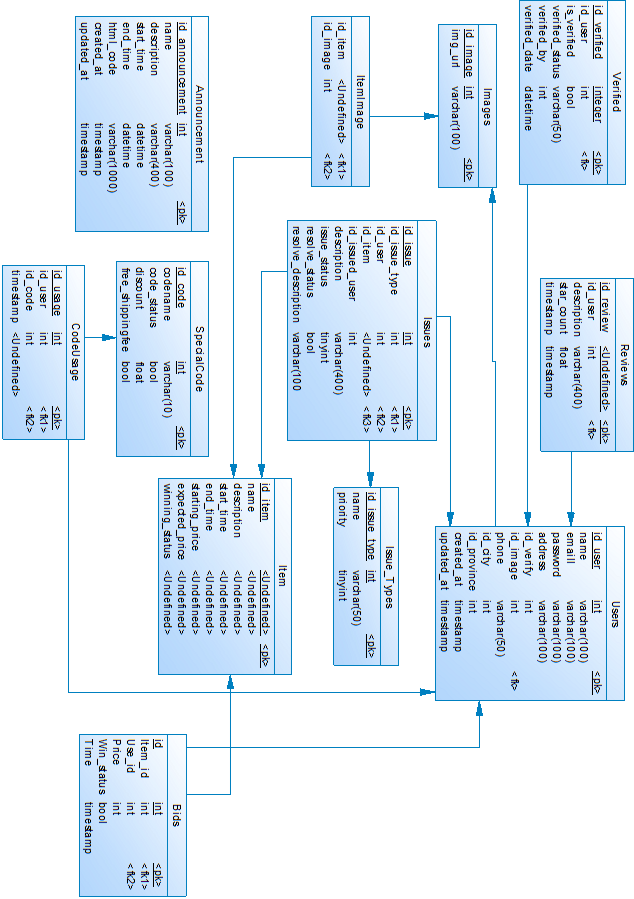
\includegraphics[height=0.6\paperheight]{images/bab3/db/pdm-awal.png}
		\caption{Rancangan Awal PDM untuk Database Relasional}
		\label{pdm-awal}
	\end{figure}
	
	Dan untuk tabel NoSQL dirancang sebagai berikut :
	\begin{figure}[H]
		\centering
		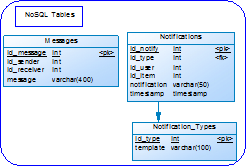
\includegraphics[width=\textwidth]{images/bab3/db/pdm-nosql-awal.png}
		\caption{Rancangan Awal PDM untuk Database Non-Relasional}
		\label{pdm-nosql-awal}
	\end{figure}
	
	\indent Dalam pengembangan aplikasi yang bersifat \textit{agile}, skema database terus diperbaiki karena perkembangan dan \textit{improvization} dari hasil analisa penulis, sehingga sifatnya menjadi dinamis.\\
	
	Berikut adalah skema database transaksional terbaru:
	\begin{figure}[H]
		\centering
		
\includegraphics[width=0.4\textheight]{images/no-image.png}
		\caption{PDM ter\textit{update} untuk Database Relasional}
		\label{pdm-final}
	\end{figure}
	
	\indent Dan Dan berikut adalah skema database non-transaksional/NoSQL terbaru:
	\begin{figure}[H]
		\centering
		
\includegraphics[width=0.4\textheight]{images/no-image.png}
		\caption{PDM Ter\textit{Update} Database Non-Relasional}
		\label{pdm-nosql-final}
	\end{figure}
	
	

	Berikut akan dipaparkan spesifikasi dan penjelasan setiap tabel.
%	\subsubsection{Spesifikasi Tabel User}
	
	\LTXtable{\textwidth}{tables/03c/users.tex}	

	